\chapter{บทนำ}

\section{ที่มาและความสำคัญ}


ในช่วงเวลาปัจจุบันนี้ เป็นช่วงที่เกิดปัญหานักศึกษาจบใหม่ว่างงานเพิ่มขึ้นทุกปี \cite{mrgonline} และมีแนวโน้มจะเพิ่มขึ้นอีกเรื่อย ๆ ซึ่งอาจส่งผลให้เกิดความเครียดในหมูนักศึกษาจบใหม่ กระทบการวางแผนชีวิตในอนาคต อาจต้องมีการย้ายสายงาน ทำงานไม่ตรงสายการเรียน เป็นต้น โดยปัญหานี้ เกิดมาจากปัจจัยหลายอย่างทั้งในแง่ระบบการปกครอง ความต้องการของสายอาชีพต่าง ๆ ในตลาดแรงงานที่เปลี่ยนแปลงไป ระบบการศึกษา หรืออื่น ๆ อีกมากมายเกินที่เราจะควบคุมได้ อย่างไรก็ตาม หากเป็นการส่งเสริมด้านการศึกษาเพิ่มเติมด้วยตัวเองและชี้แนะแนวทางนั้น สามารถเป็นไปได้ ทางคณะผู้จัดทำจึงได้เริ่มมองหาจุดที่สามารถเข้าช่วยเหลือและบรรเทาปัญหานี้ โดยเริ่มตั้งเป้าหมายไว้ที่นักศึกษามหาวิทยาลัยเทคโนโลโลยีพระจอมเกล้าธนบุรี คณะวิศวกรรมศาสตร์ สาขาวิศวกรรมคอมพิวเตอร์เป็นกลุ่มแรกก่อน เพื่อนำมาพิสูจน์ผลลัพธ์ของวิธีแก้ปัญหาที่เราออกแบบ

จากการสำรวจกับกลุ่มเป้าหมาย ทางคณะผู้จัดทำได้เล็งเห็นถึงปัญหาร่วมบางอย่าง ซึ่งทางคณะผู้จัดทำเองก็ได้ประสบพอเจอด้วยตัวเองตั้งแต่ช่วงชั้นปีที่ 1 และยังคงพบเจออยู่จนถึงปัจจุบันเช่นกัน นั่นคือปัญหาในการค้นหาและรับรู้สายอาชีพที่เหมาะสมกับตนเอง แนวทางการเรียนรู้และพัฒนาความสามารถ ไม่ทราบศาสตร์ความรู้ที่จำเป็นต่อการไปสู่สายงานนั้น ๆ เช่น วิชาเรียนที่ควรเลือกในช่วงมหาวิทยาลัย ค่ายหรืองานแข่งพัฒนาทักษะต่าง ๆ ที่ควรเข้าร่วมเพื่อเสริมประสบการณ์ แม้กระทั่งรายละเอียดหรือหน้าที่ความรับผิดชอบของสายอาชีพต่าง ๆ ก็ยังไม่เป็นที่เข้าใจอย่างถูกต้องในหมู่นักศึกษาหลายคน โดยพบว่ามีผู้ที่ประสบปัญหานี้ยังคงมีอยู่ทุกชั้นปี

จากสิ่งที่กล่าวไป ส่งผลให้นักศึกษาหลายคนไม่สามารถตอบได้ว่าตนเองควรพัฒนาตนเองอย่างไร สายอาชีพใดคือสิ่งที่ใช่สำหรับตนเอง แม้จะรู้ว่าต้องการไปในสายงานใดก็ไม่อาจทราบได้ว่าต้องพัฒนาตนเองอย่างไรต่อไปจึงจะตอบโจทย์ตลาดแรงงาน หรือรู้ตัวช้าเกินไปจนพัฒนาได้ไม่ทันการ ซึ่งสะท้อนปัญหาที่ทางคณะผู้จัดเองก็ได้พบเจอด้วย

หากสามารถแก้ไขปัญหานี้ได้ จะช่วยพัฒนาศักยภาพของนักศึกษาได้อย่างรวดเร็วและทำให้พวกขาไปถึงจุดที่ตนเองพอใจได้ง่ายขึ้น อีกทั้งยังเป็นโอกาสที่ดีในการสร้างชื่อให้แก่มหาวิทยาลัย และทำให้นักศึกษาที่สำเร็จการศึกษาสามารถใช้ช่องทางนี้ในการกลับมาเสาะหาบุคคลากรไปช่วยในตลาดแรงงานได้ในอนาคต ทำให้มีชุมชนที่แข็งแกร่งมากขึ้นตามกาลเวลา และยังช่วยให้เห็นภาพการพัฒนาตนเองที่ดียิ่งขึ้นด้วย

ทางคณะผู้จัดทำจึงมีความสนใจที่จะพัฒนาแพลตฟอร์มสำหรับใช้ช่วยเหลือในการค้นหาสายอาชีพที่เหมาะกับนักศึกษากลุ่มเป้าหมายด้วยปัญญาประดิษฐ์ พร้อมมีระบบกึ่งชุมชนที่สามารถใช้ในการให้พูดคุยเรื่องต่าง ๆ ใช้ประกาศข่าว ค้นหาเพื่อนร่วมอุดมการณ์ หรือรุ่นพี่และบุคคลในสายงานมาให้คำแนะนำนักศึกษา อีกทั้งอาจสามารถให้บุคคลภายนอกใช้ในการรับสมัครบุคลากรผ่านเว็บไซต์ได้ ทั้งในรูปแบบงานเต็มเวลาหรือการฝึกงาน ซึ่งจะช่วยให้นักศึกษาเห็นความต้องการของตลาดแรงงานตามจริง เป็นโอกาสในการหาแนวทางพัฒนาตนเองล่วงหน้าหรือการมุ่งเข้าสู่สายงานที่สนใจได้

ดังนั้น  หากคณะผู้จัดทำสามารถใช้โครงงานนี้ในการช่วยเหลือนักศึกษาคนอื่น ๆ ในปัจจุบันหรืออนาคต รวมไปถึงคณะผู้จัดทำเองได้ สิ่งนี้จะเป็นประโยชน์แก่นักศึกษาอย่างยิ่งใหญ่ในด้านการศึกษาและการทำงาน เสมือนเป็นตั๋วเบิกทางให้นักศึกษามหาวิทยาลัยเทคโนโลโลยีพระจอมเกล้าธนบุรี คณะวิศวกรรมศาสตร์ สาขาวิศวกรรมคอมพิวเตอร์ ในอนาคตหลังจากนี้ ซึ่งเป็นแรงจูงใจที่สำคัญยิ่งกับทางคณะผู้จัดทำที่พบปัญหามาด้วยตนเอง และมีอุดมการณ์อยากช่วยเหลือในด้านนี้เช่นกัน


\section{วัตถุประสงค์}

ระบุสิ่งท่ี่จะทำในโครงการ ซึ่งจะใช้สำหรับการประเมินว่าโครงงานทำสำเร็จหรือไม่

\begin{itemize}
    \item  เพื่อศึกษาและจับจุดสำคัญของข้อมูลภายในเรซูเมของนักศึกษากลุ่มเป้าหมาย
    \item  เพื่อพัฒนาโมเดลปัญญาประดิษฐ์สำหรับวิเคราะห์ข้อมูลเรซูเมของนักศึกษาออกมาเป็นอาชีพที่เหมาะสมกับตัวนักศึกษาได้
    \item  เพื่อพัฒนาเว็บแอปพลิเคชันสำหรับนำมาใช้เป็นตัวกลางในการใช้งานปัญญาประดิษฐ์ เป็นชุมชนและตัวช่วยด้านการพัฒนาตนเองของกลุ่มเป้าหมายได้
    \item  เพื่อลดปัญหาการค้นหาสิ่งที่เหมาะสมและพัฒนาตนเอง ช่วยเหลือการปรับข้อมูลเรซูเม และเป็นชุมชนแก่นักศึกษาในอนาคต
\end{itemize}


\section{ขอบเขตของโครงงาน}

ขอบเขตด้านเว็บแอปพลิเคชัน
\begin{itemize}
    \item  เว็บแอปพลิเคชันจะมุ่งเน้นสนับสนุนไปที่เพียง 2 ขนาดหน้าจอ คือ เดสก์ท็อปและมือถือ
\end{itemize}

ขอบเขตด้านปัญญาประดิษฐ์
\begin{itemize}
    \item  ผู้ใช้จะต้องกรอกข้อมูลของเรซูเมด้วยตัวเองเพื่อให้ปัญญาประดิษฐ์วิเคราะห์ผลลัพธ์เป็นวิธีหลัก
    \item  ปัญญาประดิษฐ์จะรองรับภาษาอังกฤษในการวิเคราะห์เท่านั้น
\end{itemize}

ขอบเขตด้านเนื้อหาและกลุ่มเป้าหมาย
\begin{itemize}
    \item  มุ่งเน้นไปที่นักศึกษาวิศวกรรมคอมพิวเตอร์หลักสูตรปกติ และนานาชาติ
    \item  สายอาชีพที่สนับสนุนจะประกอบด้วย 5 สายอาชีพดังนี้
    \begin{itemize}
        \item Software Engineer เช่น frontent developer, backend developer และ full-stack developer
        \item Designer เช่น UX/UI Designer
        \item Data และ AI เช่น Data Engineer, Data Science และ Data Analyst
        \item Security เช่น Data Security และ Cyber Security
        \item Cloud Management เช่น DevOps
    \end{itemize}
    เนื่องจากข้อจำกัดจากข้อมูลที่มีในปัญญาประดิษฐ์ ความนิยมของสายอาชีพนั้น ๆ ในตลาดแรงงาน \cite{springnews} และนัยยะสำคัญที่ได้มาจากกลุ่มเป้าหมาย
\end{itemize}

\section{ประโยชน์ที่คาดว่าจะได้่รับ}

ทางคณะผู้จัดทำคาดหวังเป็นอย่างยิ่งว่าจะสามารถนำเว็บแอปพลิเคชันนี้มาใช้งานกับนักศึกษาวิศวกรรมคอมพิวเตอร์ทุกชั้นปีซึ่งรวมถึงคณะผู้จัดทำเองด้วย โดยหวังว่าจะช่วยเหลือให้กลุ่มเป้าหมายนี้ สามารถปรังปรุงเรซูเมของตัวเองให้ดียิ่งขึ้น หรือปรับให้เข้ากับความต้องการของตนเอง เสริมความมั่นใจในการนำไปสมัครงานตามช่องทางที่ตนเองสนใจ รวมไปถึงใช้งานเว็บแอปพลิเคชันเพื่อพัฒนาตนเอง เสาะหาโอกาสเพิ่มเติมในสายอาชีพ รวมไปถึงกลับมาค้นหาผู้ที่สนใจร่วมงานด้วยในอนาคตหลังจบการศึกษา ซึ่งถือเป็นการสร้างชุมชนที่แข็งแกร่งขึ้นตามกาลเวลา อีกทั้งยังสามารถพัฒนาปัญญาประดิษฐ์ให้มีประสิทธิภาพมากขึ้นจากข้อมูลที่ได้รับระหว่างเปิดให้ใช้งานตามเวลาอีกด้วย ซึ่งเป็นประโยชน์อย่างมากในยุคที่ข้อมูลมีความสำคัญเช่นนี้

\section{ตารางการดำเนินงาน}
\begin{figure}[!h]\centering
    \setlength{\fboxrule}{0.2mm}
    \setlength{\fboxsep}{0.5cm}
    \fbox{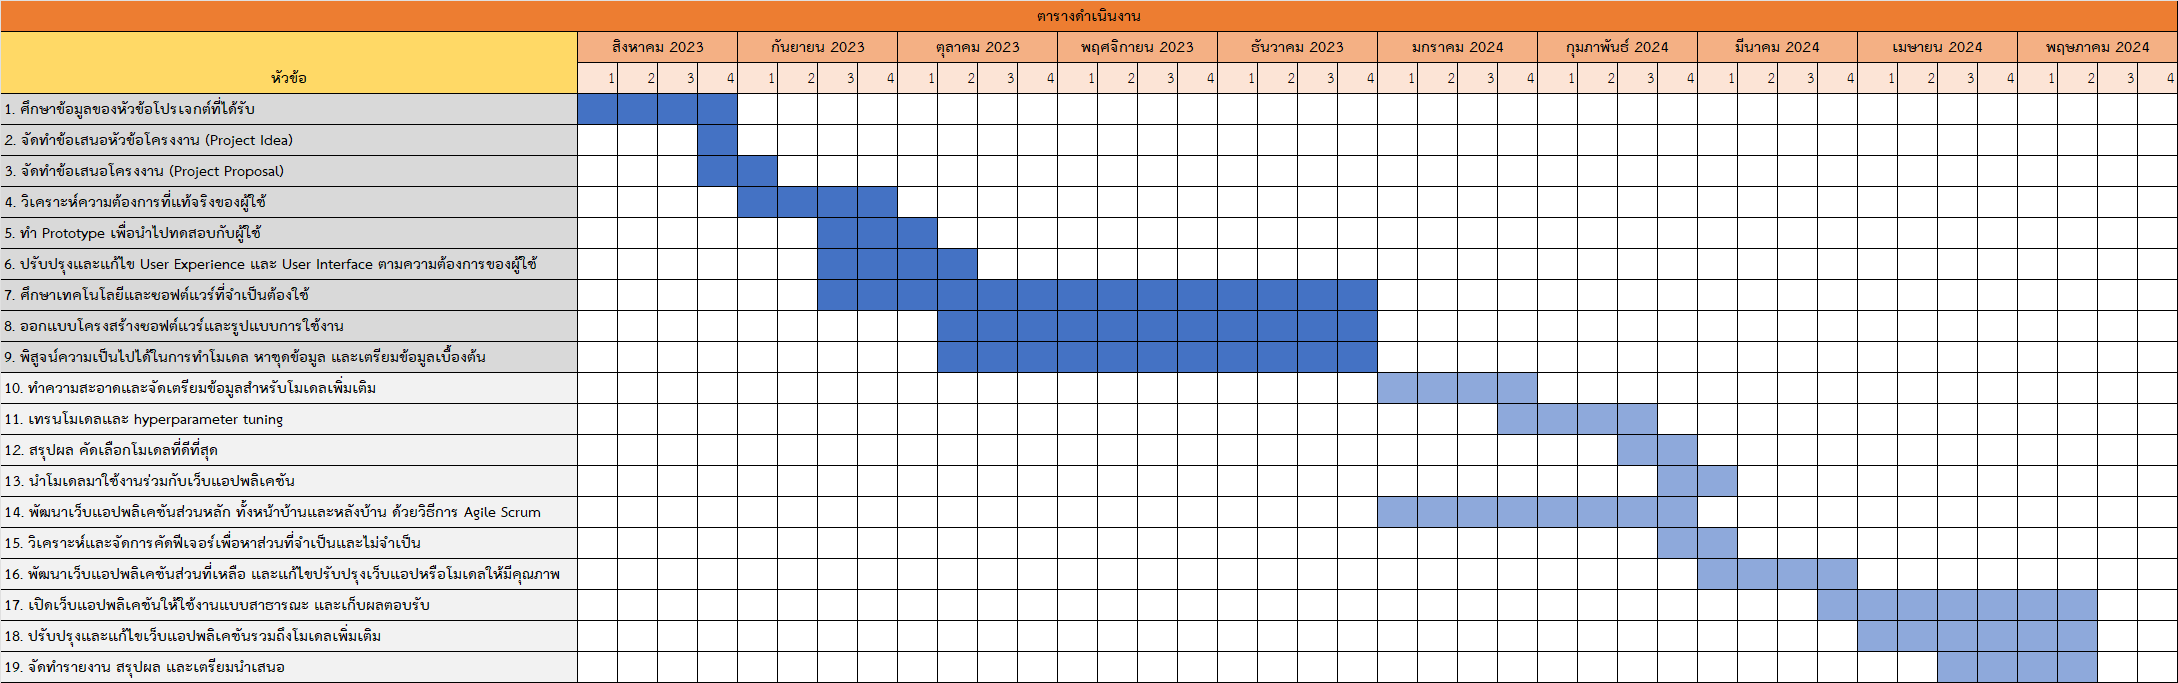
\includegraphics[width=15cm]{./figure/figure_ganttchart.png}}
    \caption{ตารางการดำเนินงาน}\label{fig:model4}
\end{figure}